\section{Isomorphismes entre protéines}
\subsection{Définition}
\begin{frame}{Définition d'un isomorphisme de graphes}
\footnotesize
\fbox{%
\begin{minipage}{0.95\textwidth}

\underline{Définiton} : Soit $A_g$=$\lbrace g_1,\cdots,g_n \rbrace$ et $A_h$=$\lbrace h_1,\cdots,h_n \rbrace$ des ensembles
\newline Soit G=$A_g \times S_g$ et H=$A_h \times S_h$ 
deux graphes où $S_g,S_h\subseteq[n]\times[n]$ 
\newline ( ainsi, l'arête $(g_i,g_j)$ est dans G $\iff (i,j)\in S_g$ ) :
\begin{equation}
G \cong H\ si\ et\ seulement\ si\
\exists \sigma \in \Sigma _n, S_g = S_h^\sigma
\end{equation}
où $S_h^\sigma := \lbrace (\sigma(i),\ \sigma(j)),\ \exists (i,j) \in [\![1,n]\!]^2,\ (i,j) \in S_h \rbrace$
\end{minipage}
}
\newline
\newline
\underline{Exemple} :
    \begin{figure}[!htb]
        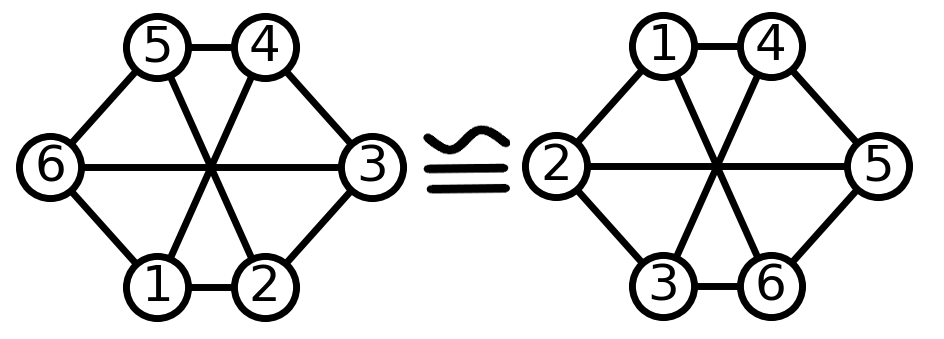
\includegraphics[width=9cm]{def_isom_ex1}
    \end{figure}
\end{frame}

\begin{frame}
    \begin{figure}[!htb]
        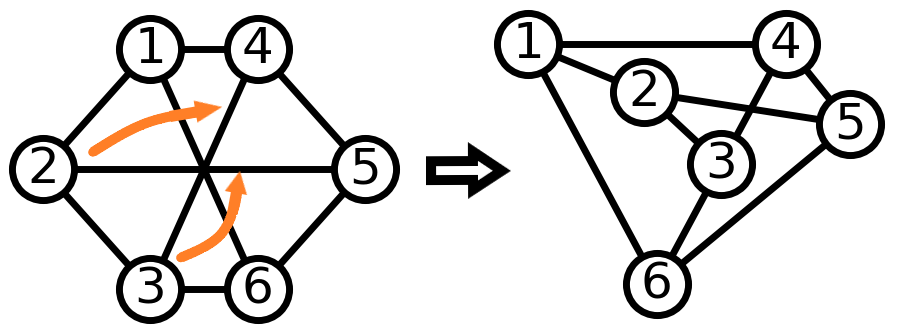
\includegraphics[width=9cm]{def_isom_ex2}
    \end{figure} 
    donc :
    \begin{figure}
        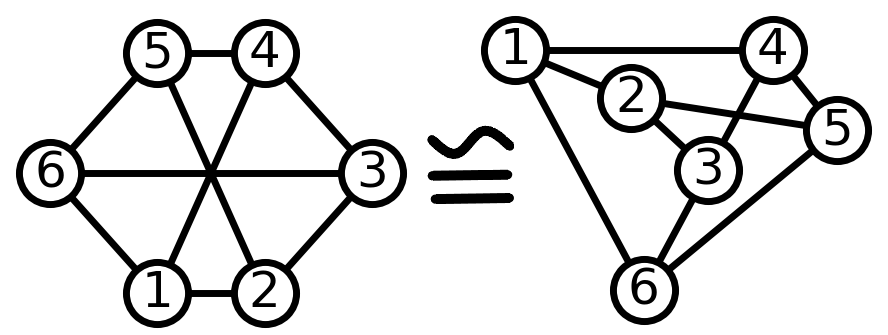
\includegraphics[width=9cm]{def_isom_ex3}
    \end{figure}
\end{frame}

\begin{frame}{Notion d'isomorphisme appliquée aux protéines}
    \small
    \begin{multicols}{3}
        \begin{figure}[!htb]
            \centering
            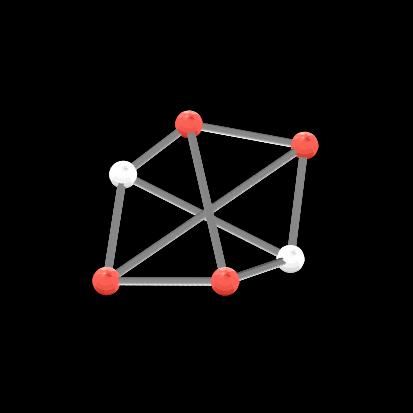
\includegraphics[width = 2.6cm]{prot_isom1}
        \end{figure}
        \begin{figure}[!htb]
            \centering
            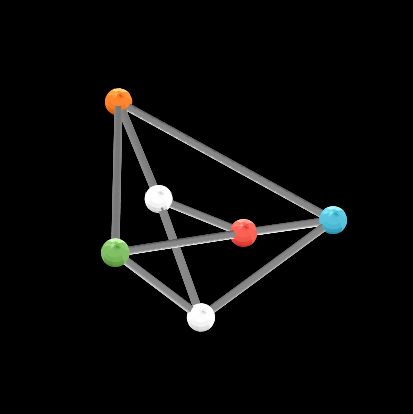
\includegraphics[width = 2.6cm]{prot_isom3}
        \end{figure}
        $\bullet$ Même structure 
        \newline $\bullet$ atomes différents
        \newline $\bullet$ positions des atomes différentes 
    \end{multicols}
    \begin{multicols}{3}
        \begin{figure}[!htb]
            \centering
            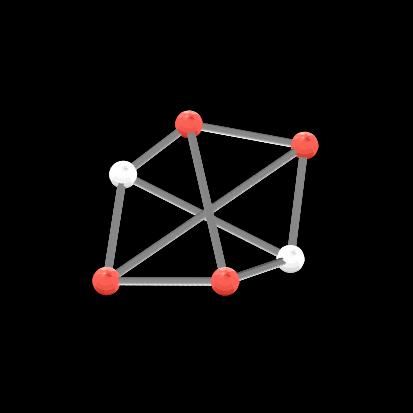
\includegraphics[width = 2.6cm]{prot_isom1}
        \end{figure}
        \begin{figure}[!htb]
            \centering
            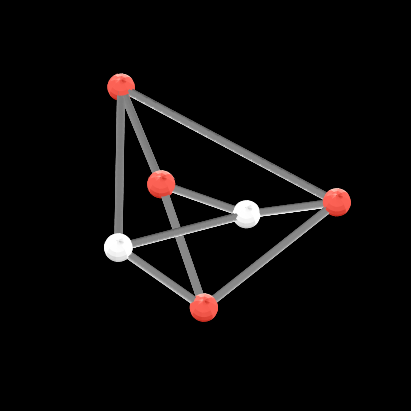
\includegraphics[width = 2.6cm]{prot_isom2}
        \end{figure}
        $\bullet$ Même structure 
        \newline $\bullet$ mêmes atomes
        \newline $\bullet$ positions des atomes différentes
    \end{multicols}
\end{frame}

\subsection{Force brute / tri des sommets}
\begin{frame}[fragile]{Idée 1 : Recherche par force brute}
\footnotesize
Pour simplifier, on considère G=$[\![ 1,n]\!]\times S_g$ et H=$[\![ 1,n]\!]\times S_h$ 
\newline\newline On cherche pour $\sigma \in \Sigma_n$, une permutation $\sigma$ telle que $S_g=S_h^\sigma$,

En python : 

\begin{itemize}
    \item type : \textcolor{charcoal}{Graph}
        \begin{tabular}{rl}
            \textcolor{airforceblue}{Graph.vertices} & $\longleftrightarrow \quad$ int list (liste des sommets) \\ 
            \textcolor{airforceblue}{Graph.edges} & $\longleftrightarrow \quad$ int list list (liste d'adjacence)
        \end{tabular}
        \newline\underline{ex} : $G_1 = Graph(\ [0,1,2],\ [[0,1], [0], [0]]\ )$
        \newline $\quad H_1 = Graph(\ [0,1,2],\ [[1,0], [2], [2]] )$
    \item type : permutation : int list
        \newline \underline{ex} : sur $\Sigma_3,\ Id = [0,1,2],\ \sigma_1=[2,1,0]$ la transpositon de 1 et 3
    \item fonction : \textcolor{airforceblue}{test$\_$isomorphism} : Graph, Graph, int list $\longrightarrow$ bool
        \newline \underline{ex} : $test\_isomorphism( G_1, H_1 , [0,1,2])$
        \newline teste si G et $H^{\sigma}$ sont les mêmes graphes
    \item fonction : \textcolor{airforceblue}{isomorphes} : Graph, Graph $\longrightarrow$ bool
        \newline \underline{ex} : $isomorphes(G, H) = True$
        \newline $G_1$ et $H_1$ sont isomorphes car $\exists \sigma \in \Sigma_3,\ (\sigma=\sigma_1)\ G_1=H_1^{\sigma}$
\end{itemize}
\end{frame}

\begin{frame}{Idée 2 : tri des sommets par invariants}
Les invariants des sommets que l'on peut utiliser sont par exemple le degré, le type du sommet,$\dots$ \newline\newline
\underline{Exemple} : G = $[\![1,5]\!] \times S_g$
\begin{align*}
\text{Les sommets ont une couleur : }
    & 1 ,\ 2\ \text{et}\ 4\ \text{sont bleus} \\
    & 3\ \text{et}\ 5\ \text{sont rouges}
\end{align*}
\begin{center}
Et ont aussi un degré égal au nombre de voisins
\end{center}
\begin{figure}[!htb]
    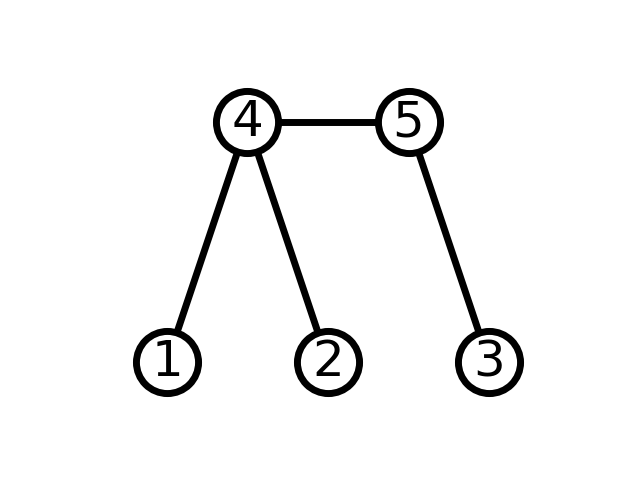
\includegraphics[width=5cm]{graph_tri.png}
\end{figure}


\end{frame}
\footnotesize
\begin{frame}
    \begin{center}
        On peut trier les sommets par couleurs : $(1\ 2\ 4\ |\ 3\ 5)$
        \begin{figure}[!htb]
        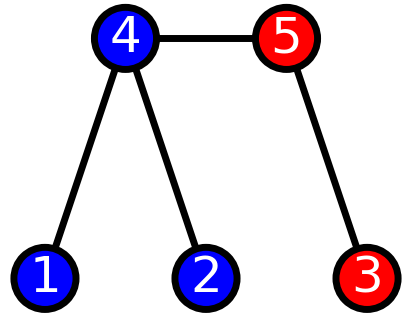
\includegraphics[width=2.5cm]{graph_tri_couleur.png}
        \end{figure}
        Ou trier les sommets par degré : $(1\ 2\ 3\ |\ 5\ |\ 4)$
        \begin{figure}[!htb]
        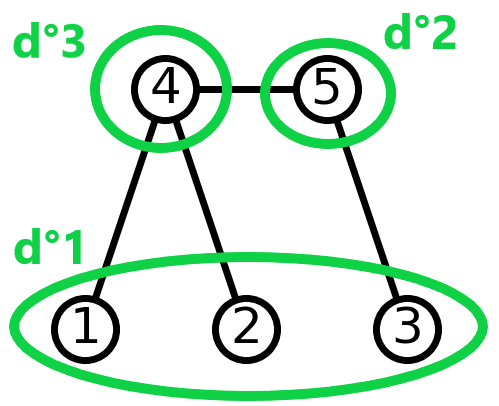
\includegraphics[width=2.8cm]{graph_tri_deg.png}
        \end{figure}
        Puis combiner les deux :  $(1\ 2\ |\ 3\ |\ 5\ |\ 4)$
        \begin{figure}[!htb]
        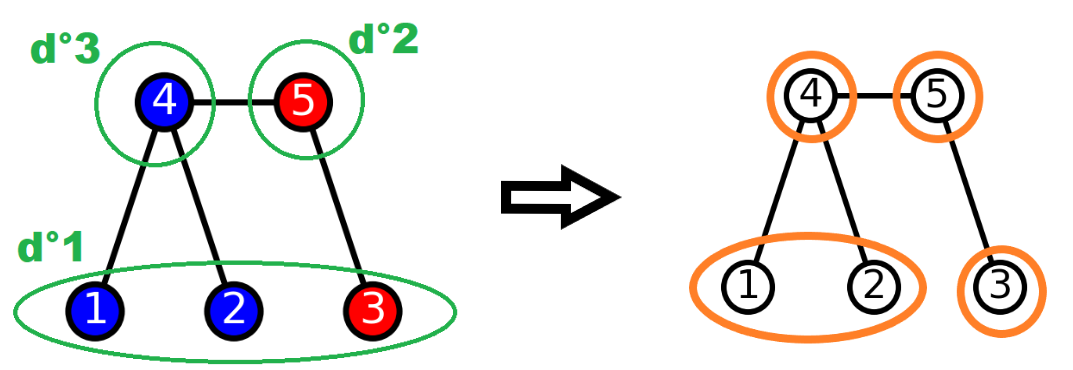
\includegraphics[width=7.1cm]{graph_tri_to_combin.png}
        \end{figure}
    \end{center}
\end{frame}

\begin{frame}{Idée 2 : tri des sommets par invariants}
Principe de recherche d'isomorphisme avec les sommets triés :
\begin{figure}[!htb]
    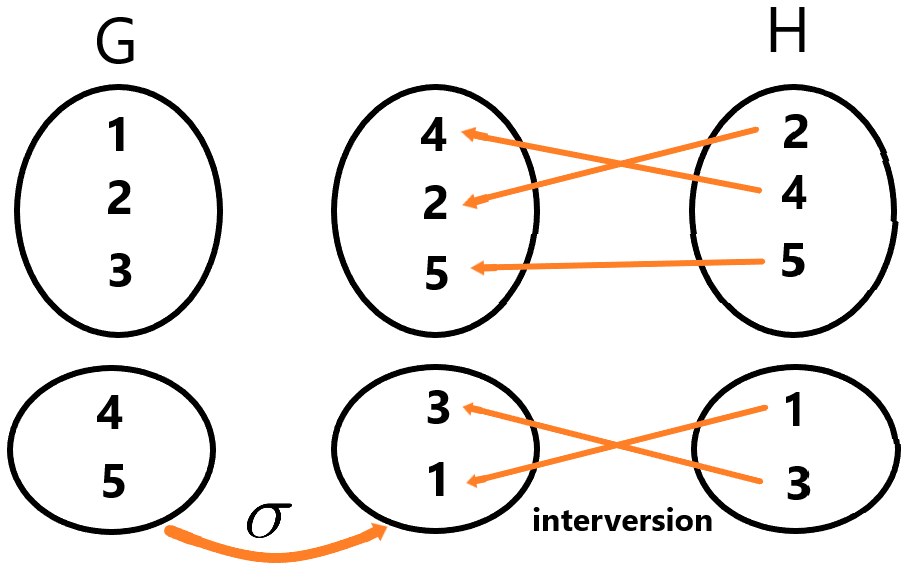
\includegraphics[width=9cm]{explication_tri.png}
    \end{figure}
\end{frame}

\begin{frame}{Idée 2 : tri des sommets par invariants}
    

\end{frame}

\begin{frame}{Tri sur les protéines}
    \begin{multicols\fbox{%
    \begin{minipage}{0.95\textwidth}
        On crée ainsi une partition de $[\![1,n]\!]$ des sommets $(V_1|\dots| V_t)$ pour G
        et $(W_1|\dots|W_t)$ pour H alors : \footnotesize
        \begin{equation}
            G \cong H \iff
            \exists (\sigma_i)_{i\in[\![ 1,t]\!]} \in 
            \Sigma _{|V_1|}\times..\times\Sigma _{|V_t|},\ 
            S_g=S_h^{\tilde{\sigma_1}\circ .. \circ \tilde{\sigma_t}}
        \end{equation} \footnotesize
        \begin{align*}
            avec\ \forall v_{i,j} \in V_i,\ \tilde{\sigma_i }(v_{i,j}) &= w_{i,\sigma_i(j)}\ 
            avec\ V_i=( v_{i,1}\ \dots\ v_{i,|V_i|} )\\
            \forall v \notin V_i,\ \tilde{\sigma_i }(v) &= v\
        \end{align*}
    \end{minipage}
    } \scriptsize \newline
\underline{Exemple} :
    \begin{align*}
        (V_1,V_2) &\to ( \quad 1 \quad 2 \quad 3 \quad| \quad 4 \quad 5\quad ) \\
        (W_1,W_2) &\to ( \quad 1 \quad 3 \quad 5 \quad| \quad 2 \quad 4\quad )
    \end{align*}
    \begin{center}
    \begin{tabular}{cccc}
        $\sigma_1$ 
        \footnote{
        $pour\ \sigma \in \Sigma_n ,\ on\ note\ \sigma = (\sigma(1)\ \sigma(2)\ \cdots\ \sigma(n)) $
        }
        & $\sigma_2$ & $(W_1^{\sigma_1}|W_2^{\sigma_2})$ & $\sigma = \tilde{\sigma_1} \circ \tilde{\sigma_2}$ \\
        \hline
        $(1\ 2\ 3)=Id$ & $(1\ 2)=Id$ & $( 1\quad 3\quad 5\ |\ 2\quad 4)$ & $(1\quad 3\quad 5\quad 2\quad 4)$ \\
        $(3\ 2\ 1)$ & $(1\ 2)=Id$ & $( 5\quad 3\quad 1\ |\ 2\quad 4)$ & $(5\quad 3\quad 1\quad 2\quad 4)$ \\
        $(1\ 2\ 3)=Id$ & $(2\ 1)$ & $( 1\quad 3\quad 5\ |\ 4\quad 2)$ & $(1\quad 3\quad 5\quad 4\quad 2)$ \\
    \end{tabular}
    \end{center}}{3}
    \begin{figure}[!htb]
        \centering
        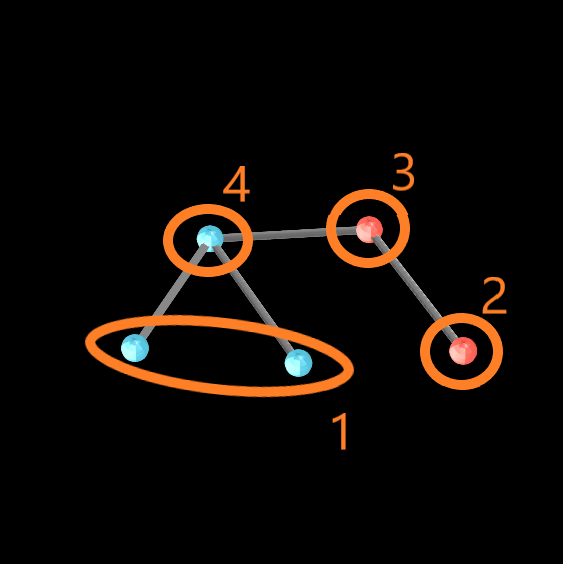
\includegraphics[width = 3cm]{prot_tri1}
    \end{figure}
    \begin{figure}[!htb]
        \centering
        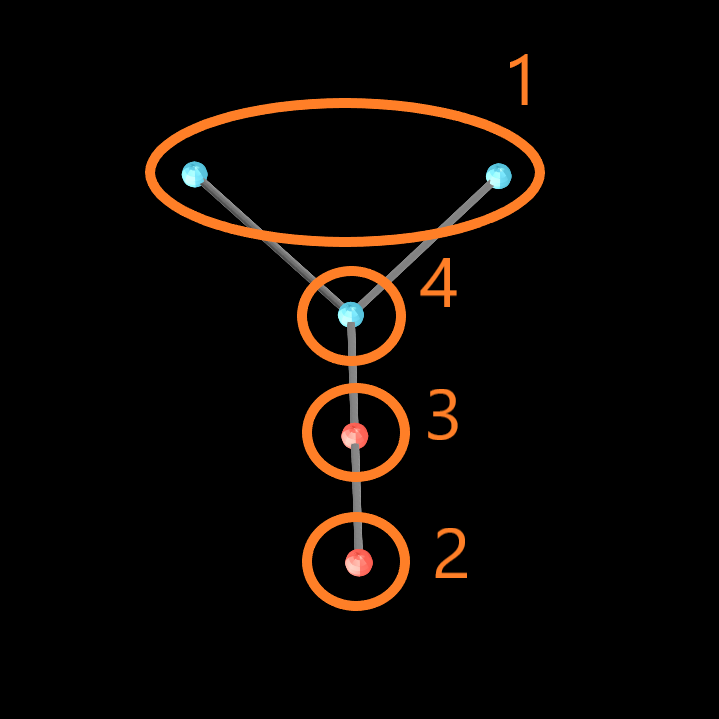
\includegraphics[width = 3cm]{prot_tri2}
    \end{figure}
    \begin{figure}[!htb]
        \centering
        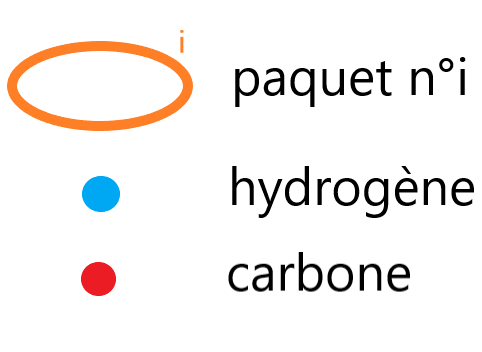
\includegraphics[width = 2cm]{legende_prot_tri}
    \end{figure}
    \end{multicols}
    \vspace*{1cm}
    \begin{minipage}{0.8\textwidth}
    \begin{center}
        \begin{tabular}{c|c|c}
            & force brute & tri \\
            \hline
            & & \\
            permutations & $5!=120$ & 2 \\
            de sommets & &
        \end{tabular}
    \end{center}
\end{minipage}
\end{frame}

\subsection{Comparaion}
\begin{frame}{Comparaison des complexités force brute / tri}
    G et H sont des graphes à n sommets tous deux \textbf{triés canoniquement}:
    \begin{itemize}
        \item types des $t \in \mathbb{N}$ paquets du tri sont dans le \textbf{même ordre} 
        \item on suppose les paquets de \textbf{même tailles} $t_i,\ i \in [\![1,t]\!]$ (sinon les graphes seraient trivialement non isomorphes)
        \newline 
    \end{itemize} 
    \scriptsize
    \begin{center}
    \begin{tabular}{c|c|c}
        & force brute & tri des sommets \\
        \hline & & \\
        procédé & permutations sur $\Sigma_n$ & combinaison de permutations sur \\
        d'itération & & $(\Sigma_i)_{i \in [\![1,t]\!]}$ tel que $\sum_{i=1}^t t_i  = n$ \\ & & \\
        \hline
        nombre & & \\ maximal & $n!$ & $\prod_{i=1}^t t_i!$ \\ d'itérations & & \\
        \hline
        mise en & & \\ mémoire & $\sum_{k=1}^n k! $ permutations & $\sum_{k=1}^{max(t_1,..,t_t)} k! $ permutations \\ nécéssaire
    \end{tabular}
    \end{center}
\end{frame}

\begin{frame}{Comparaison des complexités force brute / tri}
    On considère deux graphes triés en n paquets de taille q :
    \begin{figure}[!htb]
        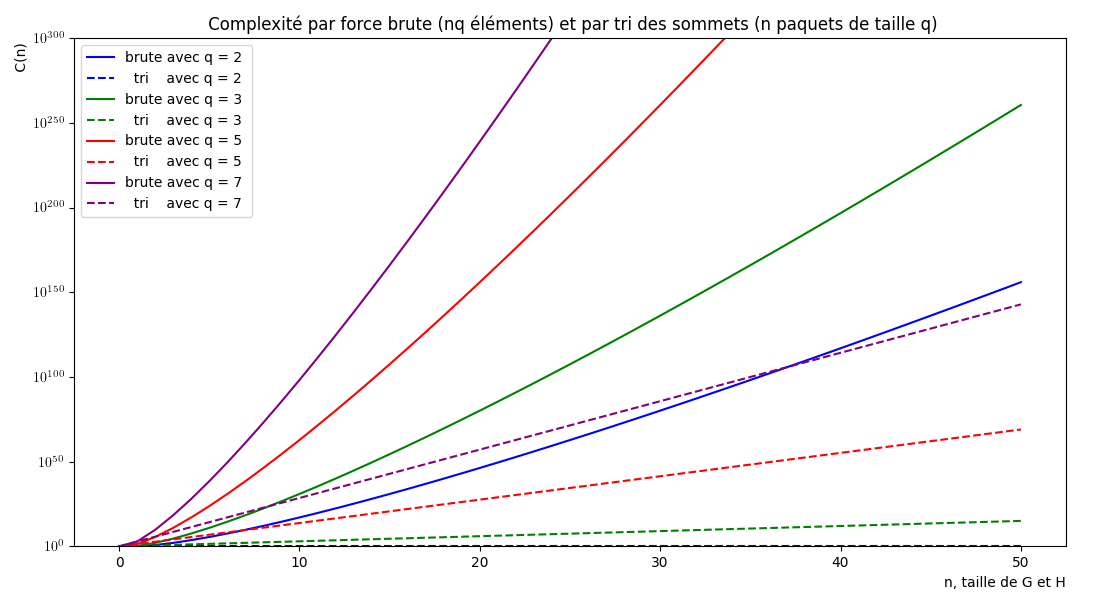
\includegraphics[width=10.3cm]{complexite_force_brute_tri_r.png}
    \end{figure}
\end{frame}